% This is LLNCS.DEM the demonstration file of
% the LaTeX macro package from Springer-Verlag
% for Lecture Notes in Computer Science,
% version 2.4 for LaTeX2e as of 16. April 2010
%
\documentclass{llncs}
%
\usepackage{makeidx} % allows for indexgeneration
\usepackage{graphicx}
\usepackage{epstopdf} %%package to overcome problem with eps in pdf files
\usepackage{subcaption}
\captionsetup{compatibility=false}
\usepackage{algorithm} 
\usepackage{algpseudocode} 
\usepackage{amsmath, bm} 
\usepackage{lipsum}
\usepackage{multirow}
\usepackage{bbding}
\usepackage[misc]{ifsym}
\usepackage[margin=4.5cm]{geometry}
\addtolength{\textheight}{1cm}
\usepackage{multicol}
\renewcommand{\algorithmicrequire}{\textbf{Input:}} % Use Input in the format of Algorithm 
\renewcommand{\algorithmicensure}{\textbf{Output:}} % Use Output in the format of Algorithm
\def\ackname{Acknowledgement.}
%
\begin{document}
%
\frontmatter % for the preliminaries
%
\pagestyle{headings} % switches on printing of running heads
\addtocmark{Hamiltonian Mechanics} % additional mark in the TOC
%
\mainmatter % start of the contributions
%
\title{Clustering of Multiple Density Peaks}
%
\titlerunning{Hamiltonian Mechanics} % abbreviated title (for running head)
% also used for the TOC unless
% \toctitle is used
%
\author{Borui Cai\inst{1\textrm{(\Letter)}} \and
Guangyan Huang\inst{1} \and
Yong Xiang \inst{1} \and
Jing He \inst{2} \and
Guang-Li Huang\inst{3} \and
Ke Deng\inst{3} \and
Xiangmin Zhou\inst{3}}
%
%\authorrunning{Ivar Ekeland et al.} % abbreviated author list (for running head)
%
%%%% list of authors for the TOC (use if author list has to be modified)
%\tocauthor{Ivar Ekeland, Roger Temam, Jeffrey Dean, David Grove,
%Craig Chambers, Kim B. Bruce, and Elisa Bertino}
%
\institute{School of Information Technology, Deakin University, Melbourne, Australia\\
\email{\{bcai,guangyan.huang,yong.xiang\}@deakin.edu.au} \\
\and
Data Science Research Institute, Swinburne University of Technology, \\
Melbourne, Australia \\
\email{lotusjing@gmail.com} \\
\and
School of Science, RMIT University, Melbourne, Australia \\
\email{guangli.huang@student.rmit.edu.au} \\
\email{\{ke.deng,xiangmin.zhou\}@rmit.edu.au}}


\maketitle % typeset the title of the contribution
\begin{abstract}
Density-based clustering, such as Density Peak Clustering (DPC) and DBSCAN, can find clusters with arbitrary shapes and have wide applications such as image processing, spatial data mining and text mining. In DBSCAN, a core point has density greater than a threshold, and can spread its cluster ID to its neighbours. However, the core points selected by one cut/threshold are too coarse to segment fine clusters that are sensitive to densities. DPC resolves this problem by finding a data point with the peak density as centre to develop a fine cluster. Unfortunately, a DPC cluster that comprises only one centre may be too fine to form a natural cluster. In this paper, we provide a novel clustering of multiple density peaks (MDPC) to find clusters with arbitrary number of regional centres with local peak densities through extending DPC. In MDPC, we generate fine seed clusters containing single density peaks, and form clusters with multiple density peaks by merging those clusters that are close to each other and have similar density distributions. Comprehensive experiments have been conducted on both synthetic and real-world datasets to demonstrate the accuracy and effectiveness of MDPC compared with DPC, DBSCAN and other base-line clustering algorithms.
\keywords{clustering, density peaks, cluster merge}
\end{abstract}
%
\section{Introduction}
Clustering can discover the relationship of points by grouping similar points into the same cluster; this capability makes it attractive in many data mining tasks. K-means finds the best $k$ centres to minimize the overall distance between the points and their centres \cite{imagekmeans}. Affinity Propagation (AP) \cite{ap} finds the best point to represent the whole cluster. However, both of them are not effective in finding non-spherical clusters. 

Mean-shift \cite{meanshift} is designed to find non-spherical clusters, but it highly relies on the significance of density gradients among data points. Density-based clustering methods, such as Density Peak Clustering (DPC) \cite{dp} and DBSCAN \cite{dbscan}, use critical data points to form clusters. DBSCAN finds natural shape clusters by finding core data points which spread cluster IDs to their neighbours; and a core point is a data point that has density greater than a threshold. However, core data points that are selected based on one cut/threshold in DBSCAN are too coarse to segment fine clusters that are sensitive to density, as shown in the third dataset in Fig.\ref{fig:three}(c), where we can only accurately find the top left clusters (two sparse clusters) or the bottom left clusters (two dense clusters), but not both. Also, in practice it is hard to find the optimal values of DBSCAN's two parameters.

DPC \cite{dp} resolves the problem of DBSCAN by finding a data point with the peak density as a centre to develop a fine cluster, and it only needs one parameter $d_{c}$, the cut-off distance. DPC converts n-dimensional features into two features: $density$ and $delta$ (the distance to the point which spreads cluster ID to it), chooses one point with the peak density as the centre for each cluster, and assigns the rest points to the relative cluster centres. DPC can find clusters with more fine densities than DBSCAN. This advantage makes DPC a potential solution to many data mining tasks \cite{imagedp,textdp}. Unfortunately, a DPC cluster that comprises only one centre (density peak) may be too fine to form a natural cluster, since this is too strict for a natural cluster that comprises multiple regional centres with local peak densities. DPC is unable to achieve a satisfying result due to two problems. First, it is difficult to choose correct cluster centres from candidate density peaks (with ``anomalously'' large $density$ and $delta$); for example, in Fig.\ref{fig:dgf}(c), although we know there are five cluster centres, it is challenging to pick them from those candidate density peaks (large red dots) in Fig.\ref{fig:dgf}(c') and requires exhaustively searching. Second, the assumption in DPC that each cluster only comprises one centre is not always true thus DPC cannot find natural shape clusters accurately; three examples are shown in Fig.\ref{fig:three}(b). 

Hierarchical clustering inspires us to merge DPC clusters and form the correct clusters that comprise multiple density peaks. We initially generate seed clusters by DPC and merge seed clusters according to their distances. Thus, a good cluster distance is the key for the accuracy. We have tested four existing cluster distances (``single'', ``average'', ``complete'' and Hausdorff linkage \cite{hausdorff}), but their accuracy is not good in merging DPC seed clusters, as shown in Fig.\ref{fig:dist}.

In this paper, we propose a novel Multiple Density Peaks Clustering (MDPC) method to flexibly find clusters with arbitrary number of regional centres that have local peak densities (as they exist in the real world) through extending DPC. In MDPC, we generate fine seed clusters, which are simpler than natural shape clusters since each seed cluster has only one density peak, and discover a natural shape cluster with multiple density peaks by merging those seed clusters that are close to each other and have similar density distributions. We conduct comprehensive experiments on both synthetic and real-world datasets to demonstrate the accuracy and effectiveness of MDPC. Therefore, this paper has three contributions:
\begin{itemize}
\item We provide a novel MDPC method, which improves DPC in two aspects: to find natural shape clusters with arbitrary number of  local density peaks and to form seed clusters by automatic selection of cluster centres.
\item We define a new measurement of the distance between two seed clusters, based on which seed clusters are merged more accurately in MDPC than four counterpart cluster distances (``single'', ``average'', ``complete'' and Hausdorf \cite{hausdorff}).
\item We conduct experiments on both synthetic and real-world datasets to prove that MDPC achieves more accurate results than DPC, DBSCAN and other baseline clustering algorithms.
\end{itemize}
The rest of this paper is organized as follows. Section 2 presents the preliminary knowledge and problem definition. Section 3 details the proposed MDPC method. Section 4 conducts experimental studies to evaluate MDPC. Finally, Section 5 concludes the paper.
%figure to demonstrate false centers
\begin{figure}[ht]
\vspace*{-.4cm}
\centering
\begin{subfigure}[t]{0.25\textwidth}
\centering
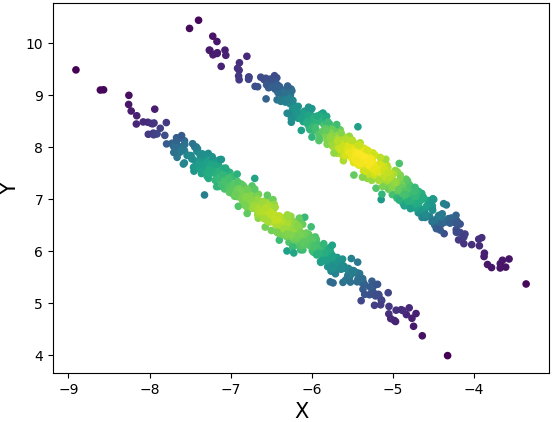
\includegraphics[width=1\textwidth]{image/dgf_org_1.png}
\subcaption*{(a)}
\end{subfigure}
\begin{subfigure}[t]{0.25\textwidth}
\centering
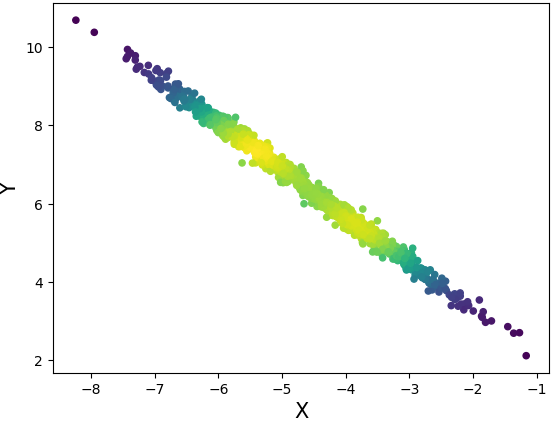
\includegraphics[width=1\textwidth]{image/dgf_org_2.png}
\subcaption*{(b)}
\end{subfigure}
\begin{subfigure}[t]{0.25\textwidth}
\centering
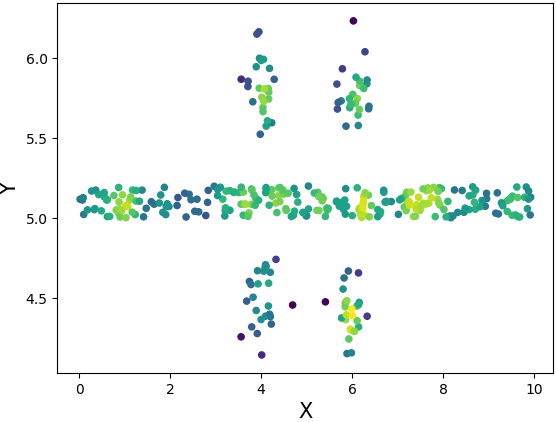
\includegraphics[width=1\textwidth]{image/dgf_org_0.png}
\subcaption*{(c)}
\end{subfigure}
\begin{subfigure}[t]{0.25\textwidth}
\centering
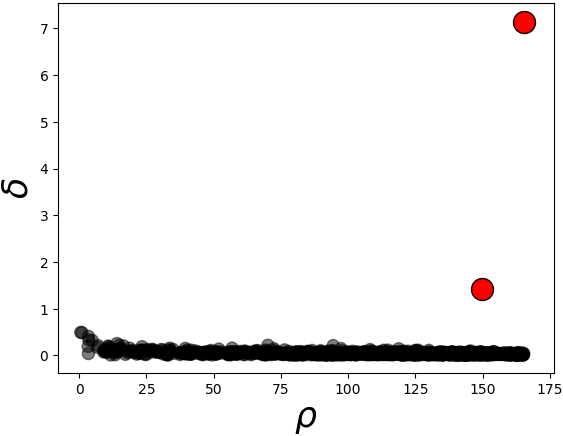
\includegraphics[width=1\textwidth]{image/dgf_dg_1.png}
\subcaption*{(a')}
\end{subfigure}
\begin{subfigure}[t]{0.25\textwidth}
\centering
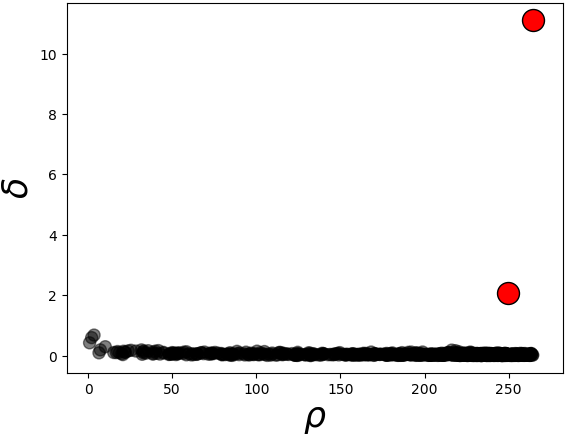
\includegraphics[width=1\textwidth]{image/dgf_dg_2.png}
\subcaption*{(b')}
\end{subfigure}
\begin{subfigure}[t]{0.25\textwidth}
\centering
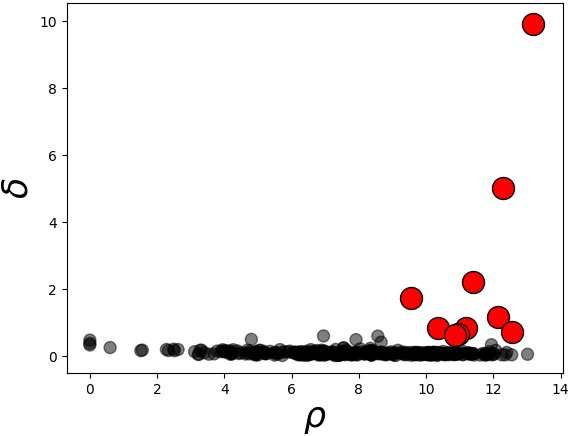
\includegraphics[width=1\textwidth]{image/dgf_dg_0.png}
\subcaption*{(c')}
\end{subfigure}
\caption{(a)-(c) are three datasets with color indicates density, and (a')-(c') are corresponding decision graphs with large red dots as candidate cluster centers.}
\label{fig:dgf}
\end{figure}
%
\section{Preliminary Knowledge and Problem Definition}
In this section, we present the DPC algorithm, point out its two problems and discuss the state of the art methods that approach these problems.
%
\subsection{The Algorithm of DPC}
%
As we mentioned in Section 1, DPC improves DBSCAN to find more fine clusters with only one density peak as a centre. That is, a DBSCAN cluster with $n$ local density peaks is possible to be split into $n$ DPC clusters. To help understand this, we introduce the main idea of DPC as follows. 
In DPC, the first step is to determine cluster centres using a $2$-dimensional ``decision graph' as follows. The $n$-dimensional feature space of a point is mapped into the $2$-dimensional feature space: $\rho$ and $\delta$. The density $\rho_{i}$ of data point $i$ is given by:
%
\begin{equation}
\rho_{i} = \Sigma_{j}\chi\left(d_{ij} - d_{c}\right),
\label{rho:normal}
\end{equation}
where $\chi\left(x\right) = 1$ if $x < 0$, and $\chi\left(x\right) = 0$ otherwise. $d_{c}$ is a threshold distance (normalized by the largest distance in this paper) and $d_{ij}$ is the Euclidean distance between data points $i$ and $j$. Then, these local density peaks are those points that have the greatest $\rho$ in its $d_{c}$ region. 
Delta $\delta_{i}$ is the minimum distance between point $i$ (with density $\rho_{i}$) and any other point, $j$, with higher density $\rho_{j}$:
%
\begin{equation}
\delta_{i} = \min_{j:\rho_{j}>\rho_{i}}\left(d_{ij}\right).
\label{delta:normal}
\end{equation}
DPC assigns the largest distance in dataset to the $\delta$ of the point with the highest density, 

In DPC, the two-dimensional features ($\rho$ and $\delta$) form a ``decision graph''; an example is shown in Fig.\ref{fig:dgf}(a'), which is transferred from raw data as shown in Fig.\ref{fig:dgf}(a). User chooses one point that has ``anomalously'' large $\rho$ and $\delta$ in decision graph \cite{dp} as the cluster centre for each cluster manually or using some heuristic ways. Then, the non-centre points are sorted in a descending order by $\rho$ and sequentially assigned the same cluster ID as their nearest point with a higher density. All data points obtain cluster IDs before DPC finds the border points whose neighbourhood cross more than one clusters.
%
\subsection{The Problems and Related Approaches}
In this paper, we will discover natural clusters that have arbitrary number of regional centres with local peak densities by extending DPC to achieve a better accuracy.
Therefore, we will tackle the two problems of DPC to satisfy this paper's goal: (1) to search for proper centres if the dataset has clusters that comprise multiple local density peaks and (2) to discover natural clusters that have multiple regional centres with local peak densities. 

If clusters contain multiple local density peaks, how to properly choose a centre for each cluster from decision graph can be difficult in DPC. As demonstrated in the dataset containing two single centre clusters as shown in Fig.\ref{fig:dgf}(a) it is intuitive to pick up two large red dots as centres in its decision graph (Fig.\ref{fig:dgf}(a')). However, the cluster with two regional centres with local peak densities in Fig.\ref{fig:dgf}(b) generates nearly identical decision graph (Fig.\ref{fig:dgf}(b')), thus the cluster may incorrectly be divided into two in DPC. 
Meanwhile in some cases, even though the number of clusters is given, it is still difficult to distinguish centres since those candidates are close to each other in the decision graph. One example is shown in Fig.\ref{fig:dgf}(c), where the large cluster in the middle contains several local density peaks. Although we know there are five clusters, it is challenging to select five centres for five clusters from the candidate large red dots in Fig.\ref{fig:dgf}(c') and requires exhaustively searching.
A recursive dividing DPC (3DC) is proposed in \cite{dgf}, but it still uses the heuristic in \cite{dp} to pick two greatest $\rho_{i}\cdot\delta_{i}$ cluster centres, which is not true in the clusters with multiple density peaks. By applying graph kernel to data vectors before inferring DPC, the candidate centres are differentiated from the common points in \cite{pakdd}, however, it still needs to choose cluster centres manually.

Even if we luckily select the right cluster centres, the non-centre local density peaks still can severely decrease the clustering accuracy. The cluster ID propagation rule of DPC is that one non-centre point obtains a cluster ID from its nearest point that has a higher density. If the nearest point with a higher density of one non-centre local density peak belongs to another cluster, this local density peak will wrongly be assigned to that cluster, and this mistake is propagated to other data points to form incorrect clusters, as shown in the three datasets in Fig.\ref{fig:three}(b). In the first dataset of Fig.\ref{fig:three}(b), the ring shape cluster is incorrectly divided into three parts and the left and right parts are assigned to the other two spherical clusters, respectively; in the second dataset, the bottom arch-shape cluster is also divided into two with the top part group with the top arch; in the third dataset, the dot shape cluster is wrongly grouped with the ring shape cluster surrounding it. 
To resolve the second problem of DPC, a two-step DPC is developed in \cite{knowledgebase2017} using the notion of core-reachable of DBSCAN. However, the merging strategy is neither well explained nor proved with convincing experiments.
%
\section{The MDPC Approach}
In this section, we present our MDPC approach that effectively finds clusters with multiple local density peaks as regional centres by two steps: 
\begin{itemize}
\item Find seed clusters. We discover the seed clusters that have single density peaks by allowing automatic selection of cluster centres.
\item Merge seed clusters. We define a new distance between seed clusters and hierarchically merge these seed clusters using this distance.
\end{itemize}

\subsection{Find Seed Clusters}
Different from DPC, natural shape clusters are regarded as the combination of several seed clusters which contain single density peaks in the scope of MDPC. That is,
all of the density peak points are centres of seed clusters. Accordingly, we define a cluster centre/density peak as follows:
\begin{equation}
c : \rho_{c} \geq \rho_{j},  dist_{ij} \leq d_{c}, \forall j \in D.
\label{link:density}
\end{equation}
%
According to Eq. (\ref{delta:normal}), the cluster centres who have peak densities in their $d_{c}$ radius have $\delta$ larger than $d_{c}$ . Accordingly, we write the list of cluster centres, $C$, as:
%
\begin{equation}
C = \{c | \delta_{c} > d_{c}, c \in D\}.
\label{link:delta}
\end{equation}
From the list of cluster centres, we find relevant seed clusters, which comprises only one density peak and satisfies the characteristic of a DPC cluster (that is, data points in a cluster coarsely following a density descending order from centre to border).

In our implementation, the DPC's original definition of density in Eq. (\ref{rho:normal}) performs not good: it either finds the unnecessary centres in a small region or incorrectly labels the non-centralized points as the cluster centres, because it regards each neighbour in $d_{c}$ region of one point the same weight without considering the distance to the centre. 
As a result, we modify the fuzzy density defined in \cite{fuzzy} as:
\begin{equation}
\rho_{i} = \Sigma_{j}\left(1 - \frac{ dist_{ij}^{2}}{d_{c}^{2}}\right),dist_{ij} \leq d_{c}, \forall j \in D.
\label{rho:fuzzy}
\end{equation}
In Fig.\ref{fig:link}, the cluster centres found by fuzzy density metric (Eq. (\ref{rho:fuzzy})) are more significant than those found by DPC density (Eq. (\ref{rho:normal})).
When $d_{c}$ is fixed, cluster centres (cross) found by the fuzzy density (Fig.\ref{fig:link}(c)-(d)) are sparser than those found by the DPC density (Fig.\ref{fig:link}(a)-(b)). Meanwhile, the fuzzy density is also more robust to $d_{c}$; the number of the cluster centres in Fig.\ref{fig:link}(a) significantly decreases when $d_{c}$ increases to 0.04, and the centre of the bottom right cluster in Fig.\ref{fig:link}(b) is lost, while the cluster centres found using fuzzy density keep stable when increasing $d_{c}$ from 0.03 (Fig.\ref{fig:link}(c)) to 0.04 (Fig.\ref{fig:link}(d)).
%
\begin{figure}[ht]
\vspace*{-.4cm}
\centering
\begin{subfigure}[t]{0.24\textwidth}
\centering
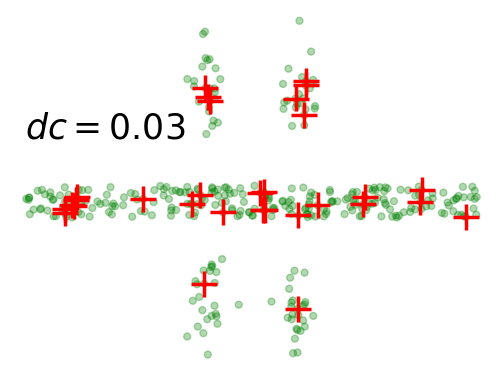
\includegraphics[width=1\textwidth]{image/003non.png}
\subcaption*{(a)}
\end{subfigure}
\begin{subfigure}[t]{0.24\textwidth}
\centering
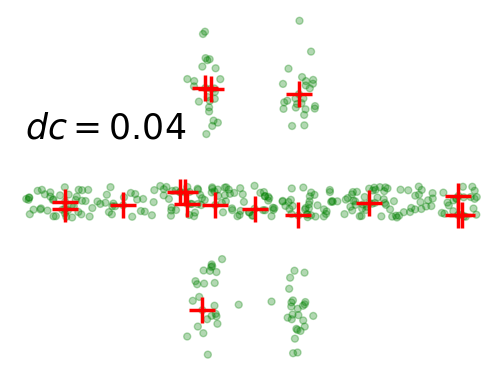
\includegraphics[width=1\textwidth]{image/004non.png}
\subcaption*{(b)}
\end{subfigure}
\begin{subfigure}[t]{0.24\textwidth}
\centering
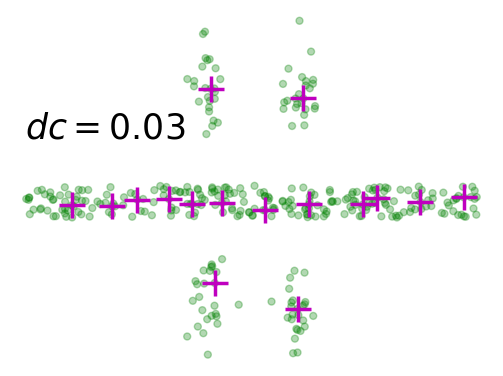
\includegraphics[width=1\textwidth]{image/003nl.png}
\subcaption*{(c)}
\end{subfigure}
\begin{subfigure}[t]{0.24\textwidth}
\centering
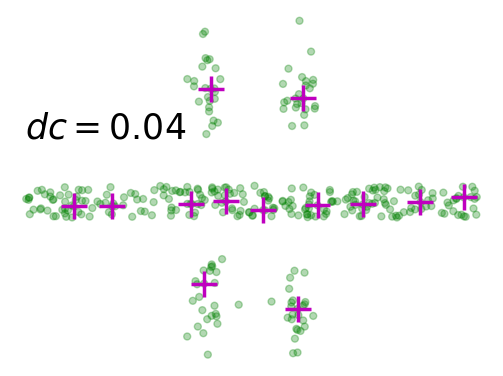
\includegraphics[width=1\textwidth]{image/004nl.png}
\subcaption*{(d)}
\end{subfigure}
\caption{Centres (colored cross) discovered by original density ((a)-(b)), and fuzzy density ((c)-(d)), with $d_{c}$ as the cut-off distance.}
\label{fig:link}
\end{figure}
The pseudocode of finding seed clusters is shown in Algorithm \ref{alg:link}. We calculate $\rho$ and $\delta$ of each data point at lines 1-7 and discover those cluster centres at line 6. Then we find seed cluster centres and assign cluster IDs to the non-centre data points at lines 8-13.
%
\begin{algorithm}[htb] 
\vspace*{-.4cm}
\caption{Find Seed Clusters ($n_{i}$: nearest point with a higher density)} 
\begin{multicols}{2}
\label{alg:link} 
\begin{algorithmic}[1] 
\Require 
Dataset $D$, 
Cutoff distance $d_{c}$
\For{each $i\in D$} 
\State Calculate $\rho_{i}$ Eq. (\ref{rho:fuzzy})
\EndFor
\For{each $i\in D$} 
\State Calculate $\delta_{i}$ by Eq. (\ref{delta:normal}), get $n_{i}$
\State Add $i$ into $C$ if $\delta_{i}$ $>$ $d_{c}$
\EndFor
\State Sort $D$ in descending order of $\rho$
\For{each $i\in D$} 
\If {$i$ $in$ $C$} $clusterID_{i}$ = new id
\Else{} $clusterID_{i}$ = $clusterID_{n_{i}}$
\EndIf 
\EndFor 
\Ensure points $clusterID$
\end{algorithmic} 
\end{multicols}
\vspace*{-.4cm}
\end{algorithm}
%
\subsection{Merge Seed Clusters}
Borrowing the idea from hierarchical clustering, we iteratively merge those seed clusters. In our MDPC, merging is conducted only on two clusters which have border regions (mutually have border points whose neighbourhood cross the two clusters). We need to define a new distance metric to achieve an effective merging since the wide-used linkage distances are too coarse for these fine seed clusters. First, two rules are defined to determine whether the seed clusters should be merged based on the characteristic of these seed clusters:
\begin{itemize}
\item Rule 1: Two clusters should be merged together if they have comparable scales and spatially close border points, as exhibited in Fig.\ref{fig:dgf}(b).
\item Rule 2: One small seed cluster should be absorbed by a larger cluster, if its scale is similar to the border region of the larger cluster and have spatially close border regions.
\end{itemize}
A seed cluster in MDPC has a coarsely monotonic density distribution in a descending order from its centre to border. Based on this characteristic and the above two rules, we define a new cluster distance by both their density distributions and their spatial distance.
As a density-based metric, our cluster distance should define the comparable scale in Rule 1 by measuring their difference of density distributions. If the density is monotonic, this difference can be defined on two aspects: the average density and the density-descending rate. Given two seed clusters A and B with average density $\rho^{A}_{avg}$ and $\rho^{B}_{avg}$, the distance between the average densities of A and B is: 
\begin{equation}
d_{merge} = \frac{\|\rho^{A}_{avg} - \rho^{B}_{avg}\|}{max\left(\rho^{A}_{avg} , \rho^{B}_{avg}\right)}.
\label{eq:S}
\end{equation}
Similarly, in Rule 2, we define the cluster distance to be the difference of the density distributions of the smaller cluster and the border region of the larger one. Assuming $A$ absorbs $B$ ($\rho^{A}_{avg}$ $>$ $\rho^{B}_{avg}$), and the border region of $A$, $border^{A}$  is defined as $\{i | dist(i,j)<d_{c}, i\in A, j \in B\}$. Thus $\rho b^{A}_{avg}$, the average density of $border^{A}$, is calculated as the average density of points in $border^{A}$ together with their neighbours. In this way, the distance between $\rho b^{A}_{avg}$ and $\rho^{B}_{avg}$ is defined as:
\begin{equation}
d_{absorb} = \frac{\|\rho b^{A}_{avg} - \rho^{B}_{avg}\|}{max\left(\rho b^{A}_{avg} , \rho^{B}_{avg}\right)}.
\label{eq:d^{AB}}
\end{equation}
We normalize the above distances and enable them to be combined together and get the overall measurement as $d_{density}$: 
\begin{equation}
d_{density} = min\left(d_{merge} , d_{absorb}\right).
\label{eq:d_{final}}
\end{equation}

The distance of the density descending rate and the spatial closeness of the cluster borders are measured by $d_{border}$, with the density of cluster centre denoted as $\rho_{c}$ and the density descending rate from the cluster centre to point $i$ as $r_{i} = \frac{\rho_{c}}{\rho_{i}}$.
\begin{equation}
d_{border} = \inf_{i \in border^{A}, j \in border^{B}}\frac{d_{ij}}{2d_{c}}\times\left(r^{A}_{i} + r^{B}_{j}\right)\|r^{A}_{i} - r^{B}_{j}\|.
\label{eq:S_{border}}
\end{equation}
We calculate $d_{border}$ to satisfy (1) $A$ and $B$ is spatial close if one point in $B$ falls in the $d_{c}$ region of $A$'s centre; (2) when one point of $B$ falls in the $d_{c}$ region of $A$'s border point, note that the border has smaller density and thus their distance must be proportionally smaller to compensate the density difference. Also, the larger the density of a pair of border points (one from $A$ and the other from $B$), the more likely these two border points are changed into inner points by merging the two clusters.
We explain how the new metric can measure the difference of the density descending rates and clusters' spatial closeness as follows. If two clusters are not close to each other, that means the distance of the border points pair $d_{ij}$ is great then makes $d_{border}$ great. A greater value of $\|r^{A}_{i} - r^{B}_{j}\|$ means their density descending rates are more different. In addition, we prefer to merge those clusters whose border points have greater densities (i.e., the value of $\left(r^{A}_{i} + r^{B}_{j}\right)$ is small).
Combining the above density distance $S_{density}$ with border distance $S_{border}$ the total distance of two seed clusters is:
%
\begin{equation}
d_{AB} = d_{border} \times exp\left(d_{density}\right),
\label{eq:distance}
\end{equation}
where $d_{AB}$ is non-negative and symmetric, and exponential (exp) is used to ensure that $d_{AB}$ is sensitive to small density variation and prevent merging of two clusters if their densities are globally distinctive even though they are spatially close.

Using the $d_{AB}$ in Eq. (\ref{eq:distance}) to measure the distance of two seed clusters, we develop a hierarchical merging algorithm (Algorithm \ref{alg:aggregate}) to form the final clusters with arbitrary numbers of density peaks. We calculate the distances of pairs of seed clusters and sort them in an ascending order at lines 1-7. Then, we merge those with distances under a threshold and re-assign new cluster IDs to all the data points at lines 8-15. Results of each iteration are recorded into a result list at line 17. 
%
\begin{algorithm}[htb] 
\caption{Hierarchical Merging of Seed Clusters ($dists$: cluster distance list)} 
\vspace*{-.4cm}
\begin{multicols}{2}
\label{alg:aggregate} 
\begin{algorithmic}[1] 
\Require 
Seed clusters $C_{seed}$
\For{seed clusters pair $a,b \in C_{seed}$}
\If {$a$, $b$ has border points}
\State calculate $d^{ab}$ with (\ref{eq:distance})
\State add $d^{ab}$ into $dists$
\EndIf 
\EndFor
\State Sort $dists$ in ascending order;
\For{each $d \in dists$}
\State Init. $clusterID_{merge}$ = $\bm{0}$;
\For{seed cluster pair $a, b\in C_{seed}$} 
\If {$d^{ij} \leq d$} merge $a$ $b$ 
\EndIf 
\EndFor
\State $clusterID_{merge}$ = merged IDs;
\State add $clusterID_{merge}$ into $L$;
\EndFor
\Ensure 
Points cluster IDs list $L$ 
\end{algorithmic} 
\end{multicols}
\vspace*{-.4cm}
\end{algorithm}

We use an example dataset \cite{dphmdataset} in Fig.\ref{fig:MDPC}(a) to explain how MDPC works. Fig.\ref{fig:MDPC}(b) are the generated seed clusters; the horizontal cluster in the middle comprises twelve seed clusters (i.e., twelve density peaks). Fig.\ref{fig:MDPC}(c) shows that the twelve seed clusters are correctly merged into one cluster.
%
\begin{figure}[ht]
\vspace*{-.4cm}
\centering
\begin{subfigure}[t]{0.28\textwidth}
\centering
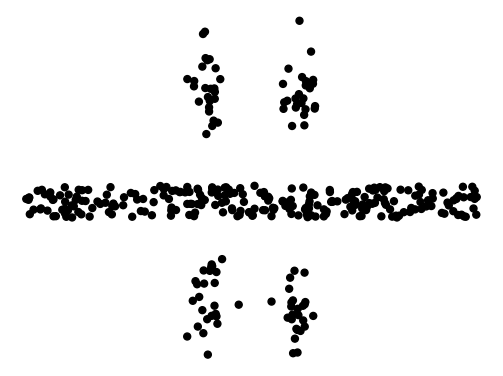
\includegraphics[width=1\textwidth]{image/org.png}
\subcaption*{(a)}
\end{subfigure}
\quad
\begin{subfigure}[t]{0.28\textwidth}
\centering
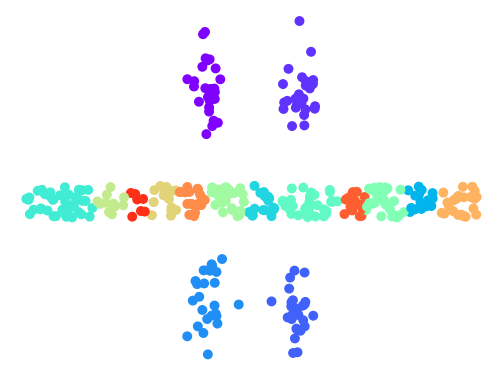
\includegraphics[width=1\textwidth]{image/no_merge.png}
\subcaption*{(b)}
\end{subfigure}
\quad
\begin{subfigure}[t]{0.28\textwidth}
\centering
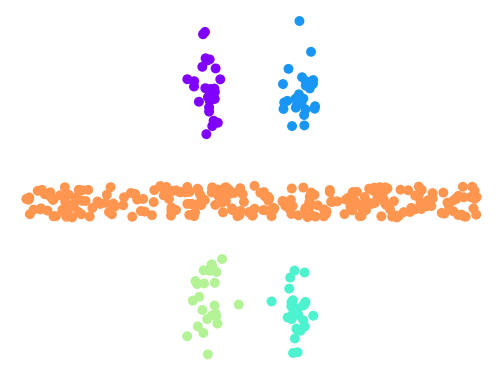
\includegraphics[width=1\textwidth]{image/correct.png}
\subcaption*{(c)}
\end{subfigure}
\caption{(a) is the original dataset, (b) and (c) shows the seed clusters found in step one and the final result in step two, respectively.}
\label{fig:MDPC}
\end{figure}
%
\subsection{Algorithm Complexity}
We denote the number of neighbours of each point as $N_{dc}$ regarding to $d_{c}$, the size of border point as $N_{b}$, and $N_{s}$ as the number of seed cluster pairs that mutually have border points, in practice, $N_{dc}$, $ N_{b}$ and $N_{s}$ are far less than the dataset size, $N$. The time complexity of finding seed clusters (Algorithm \ref{alg:link}) and border points is $O\left(2N\log{N} + N\times N_{dc} + N\right)$. The time complexity of calculating the average densities of all seed clusters is $O\left(N\right)$, and the complexity of calculating all average border densities is $O\left(N_{b}\right)$. $O\left(N_{s} + N_{s}\log{N_{s}}\right)$ is spent to compute and sort distances of seed cluster pairs, and $O\left(N_{s}\right)$ is spent on hierarchical merging. Thus, the overall time complexity of merging seed clusters (Algorithm \ref{alg:aggregate}) is $O\left(N + N_{b} + 2N_{s} + N_{s}\log{N_{s}}\right)$.
%
\section{Experiments}
In this section, we use various datasets including both synthetic datasets (four shape datasets and two density datasets) and one real-world dataset to evaluate the accuracy of our MDPC. Accuracy is measured using Normalized Mutual Information (NMI) \cite{nmi}. All algorithms, including both the proposed MDPC and the counterpart methods (DPC, DBSCAN, K-means, AP and mean-shift), are compared using the best performance under the optimal values of their parameters. We use the heuristic $\rho \times \delta$ in \cite{dp} to select the optimal cluster centres for DPC and we automatically search the best NMI of our MDPC from its output list. All the algorithms are implemented in Python 3.2 (with packages scikit-learn, numpy) and experiments are run on Windows 10 with 3.4GHz CPU and 16GB RAM. 
%
\subsection{Synthetic Datasets}
We use six different synthetic datasets with true labels. Four shape datasets with natural shape clusters (shape datasets) are Pathbased \cite{pathbased}, Jain \cite{jain}, Flame \cite{flame} and Spiral \cite{pathbased}. Two datasets with uneven density-pattern clusters (density datasets) are Compound \cite{compound} and Aggregation \cite{aggregation}. We evaluate the proposed cluster distance by comparing with four counterpart cluster distances (``single'', ``average'', ``complete'' and Hausdorff \cite{hausdorff}). We set the same experimental environment by replacing our proposed cluster distance with each of the four in MDPC. In Fig.\ref{fig:dist}, we can see that our proposed cluster distance achieves the best accuracy compared to the other four distances in all of the six datasets. The best performance improvement of the proposed distance for MDPC is in Flame, where the accuracy of the proposed method
wins the best of the other four distances (Single) by 1.000 to 0.521.
\begin{figure}[ht]
\vspace*{-.4cm}
\centering
\begin{subfigure}[t]{1\textwidth}
\centering
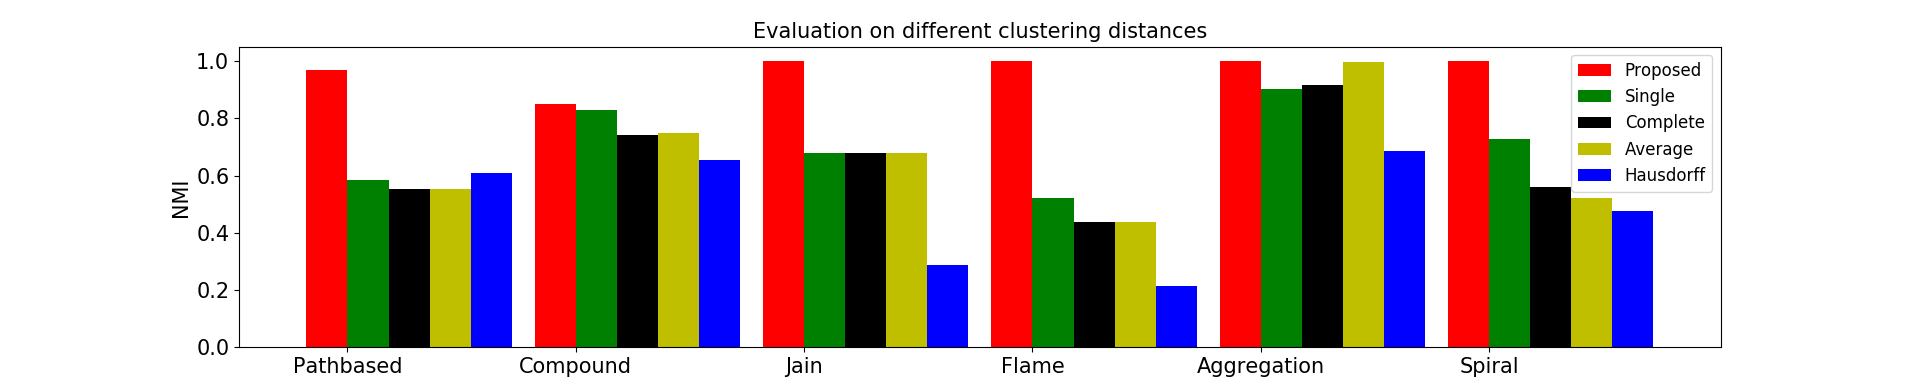
\includegraphics[width=1\textwidth]{image/distances.png}
\end{subfigure}
\caption{Evaluation of the cluster distance of MDPC with four cluster distances.}
\label{fig:dist}
\end{figure}

We compare our MDPC with two other density-based methods (DPC and DBSCAN) using three challenging datasets containing natural shape clusters with multiple local density peaks (Pathbased, Jain and Compound) (Fig.\ref{fig:three}). We can see from the first row that MDPC achieves the best accuracy in the Pathbased dataset, where both DPC and DBSCAN incorrectly split the ring shape cluster into three and two parts, respectively. In Jain dataset as shown in the second row, MDPC correctly separates the two arch-shaped clusters, while DPC incorrectly divides the bottom arch-shaped cluster into two clusters and wrongly assigns the upper cluster to the other arch-shaped cluster and DBSCAN wrongly splits the top arch-shaped cluster into two parts. In Compound dataset at the last row, only MDPC successfully finds both the two clusters (a ring and a dot the middle of the ring) at the bottom left and two spatial close round-shaped clusters at the top left, while DBSCAN only can correctly identify the two dense clusters at the bottom left or the two close sparse round-shaped clusters but not both since its one cut/threshold strategy cannot adapt itself to the clusters with different density patterns. 
\begin{figure}[ht]
\vspace*{-.4cm}
\centering
\begin{subfigure}[t]{0.23\textwidth}
\centering
\includegraphics[width=1\textwidth]{image/pathbased_MDPC.png}
\end{subfigure}
\begin{subfigure}[t]{0.23\textwidth}
\centering
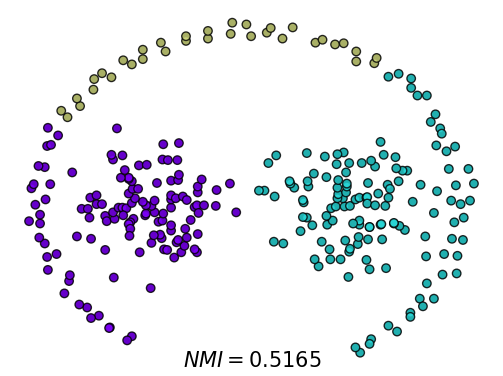
\includegraphics[width=1\textwidth]{image/pathbased_org.png}
\end{subfigure}
\begin{subfigure}[t]{0.23\textwidth}
\centering
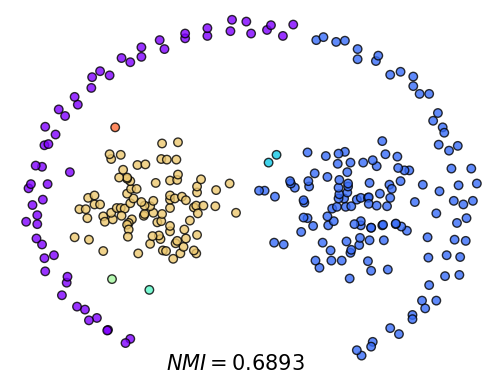
\includegraphics[width=1\textwidth]{image/pathbased_dbscan.png}
\end{subfigure}
\quad
\quad
\quad
\quad
\begin{subfigure}[t]{0.23\textwidth}
\centering
\includegraphics[width=1\textwidth]{image/jain_MDPC.png}
\end{subfigure}
\begin{subfigure}[t]{0.23\textwidth}
\centering
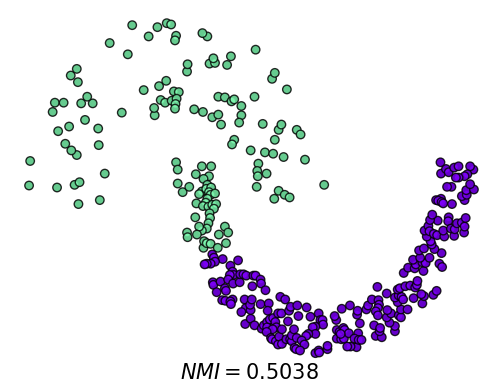
\includegraphics[width=1\textwidth]{image/jain_org.png}
\end{subfigure}
\begin{subfigure}[t]{0.23\textwidth}
\centering
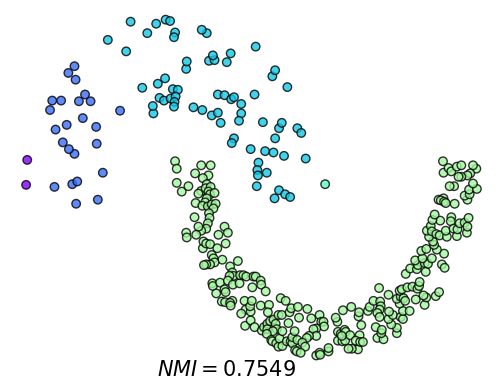
\includegraphics[width=1\textwidth]{image/jain_dbscan.png}
\end{subfigure}
\quad
\quad
\quad
\quad
\begin{subfigure}[t]{0.23\textwidth}
\centering
\includegraphics[width=1\textwidth]{image/Compound_MDPC.png}
\subcaption*{(a) MDPC}
\end{subfigure}
\begin{subfigure}[t]{0.23\textwidth}
\centering
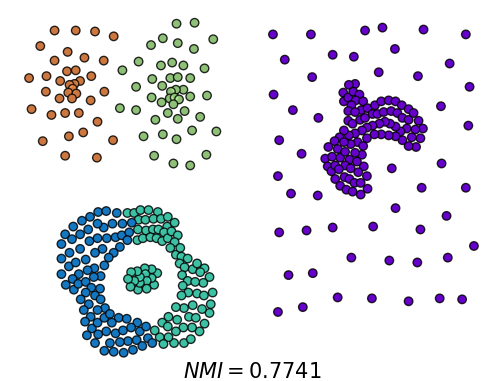
\includegraphics[width=1\textwidth]{image/Compound_org.png}
\subcaption*{(b) DPC}
\end{subfigure}
\begin{subfigure}[t]{0.23\textwidth}
\centering
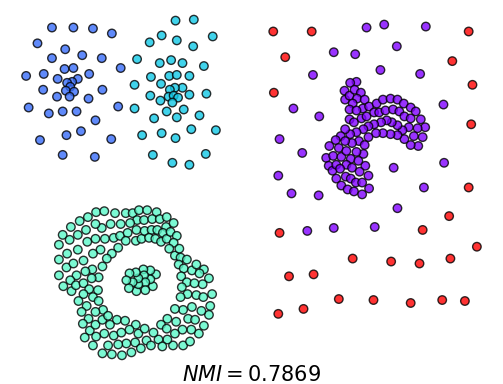
\includegraphics[width=1\textwidth]{image/Compound_dbscan.png}
\subcaption*{(c) DBSCAN}
\end{subfigure}
\caption{(a)-(c) are the clustering results of MDPC, DPC and DBSCAN, respectively.}
\label{fig:three}
\end{figure}

We also evaluate the scalability of MDPC by comparing with both density-based clustering methods (DPC and DBSCAN) and other popular ones (K-means, Affinity Propagation (AP) and mean-shift) using all of the six datasets (Table \ref{tab:synthetic}). The overall trend is that the three density-based clustering methods, MDPC, DPC and DBSCAN, perform better than the three non-density-based clustering methods. We can see from Table \ref{fig:three} that MDPC excels both DPC and DBSCAN in all of the six datasets, while DPC performs better than DBSCAN in Flame and Aggregation and DBSCAN performs better than DPC in Pathbased, Jain and Compound. This validates that our MDPC is more adaptive to density sensitive datasets than too coarse clustering in DBSCAN and too fine clustering in DPC. 
\begin{table}
\vspace*{-.4cm}
\caption{NMI on six synthetic datasets, with the best in bold and negative as `-'. }
\begin{center}
\begin{tabular}{l|l|l|l|l|l|l|l}
\hline Type &Dataset & MDPC& DPC & DBSCAN & K-means & AP & mean-shift\\
\hline \multirow{4}{*}{Shape} &Pathbased & $\bm{0.9579}$ & 0.5165 & 0.6893 & 0.5102 & 0.3530 & 0.5431\\
&Jain & $\bm{1.0000}$ & 0.5038 & 0.7549 & 0.3362 & 0.2073 & 0.3282\\
&Flame & $\bm{1.0000}$ & $\bm{1.0000}$ & 0.8654 & 0.4478 & 0.3011 & 0.4442\\
&Spiral & $\bm{1.0000}$ & $\bm{1.0000}$ & $\bm{1.0000}$ & - & 0.3142 & 0.2767\\
\hline \multirow{2}{*}{Density} &Compound & $\bm{0.8277}$ & 0.7482 & 0.7869 & 0.7421 & 0.5289 & 0.8110\\
&Aggregation & $\bm{1.0000}$ & $\bm{1.0000}$ & 0.9787 & 0.8376 & 0.5035 & 0.8983\\
\hline
\end{tabular}
\end{center}
\label{tab:synthetic}
\end{table}
%
\subsection{Real Datasets}
We use the iris dataset (with four features and three labels) from the real-world dataset UCI \cite{iris} to evaluate the accuracy of the three density-based clustering methods (MDPC, DPC and DBSAN). We use PCA to map the original four features into three features for visualization. From the result in Fig.\ref{fig:iris}, we can see that the number of mislabelled items (marked in red color) by MDPC in Fig.\ref{fig:iris}(a) is significantly less than both DPC in Fig.\ref{fig:iris}(b) and DBSCAN in Fig.\ref{fig:iris}(c) where DBSCAN wrongly groups the three categories into only two clusters.
%
\begin{figure}[ht]
\vspace*{-.4cm}
\centering
\begin{subfigure}[t]{0.32\textwidth}
\centering
\includegraphics[width=1\textwidth]{image/iris_MDPC.png}
\subcaption*{(a) MDPC}
\end{subfigure}
\begin{subfigure}[t]{0.32\textwidth}
\centering
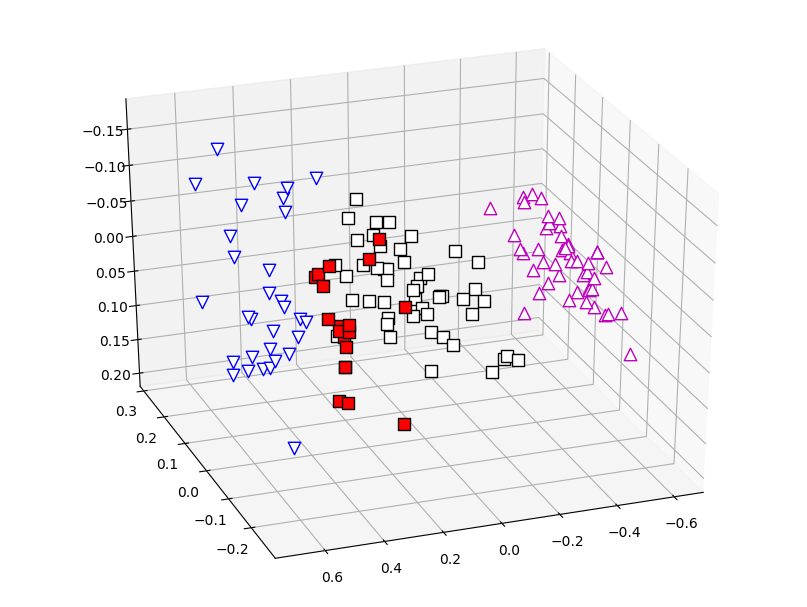
\includegraphics[width=1\textwidth]{image/iris_dp.png}
\subcaption*{(b) DPC}
\end{subfigure}
\begin{subfigure}[t]{0.32\textwidth}
\centering
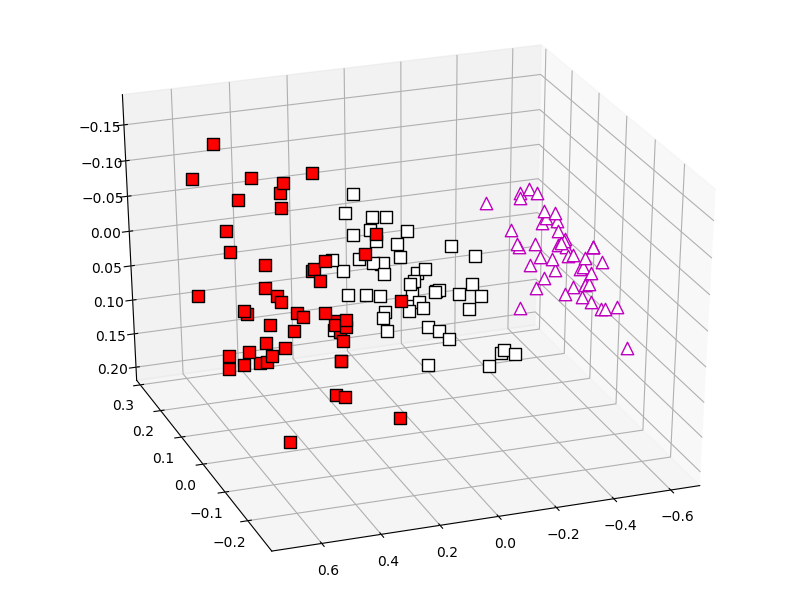
\includegraphics[width=1\textwidth]{image/iris_dbscan.png}
\subcaption*{(c) DBSCAN}
\end{subfigure}
\caption{Clustering results for the iris dataset, (a)-(c) correspond to MDPC, DPC and DBSCAN. Incorrectly clustered points are in red color.}
\label{fig:iris}
\end{figure}
%
\section{Conclusion}
In this paper, we provide the MDPC clustering method for shape and density sensitive datasets. MDPC overcomes the two problems of DPC by automatically selecting cluster centres and finding natural shape clusters with multiple local density peaks. Extensive experiments based on both synthetic and real-world datasets have demonstrated that our MDPC is a more adaptive clustering method for density sensitive datasets, compared with too coarse clustering in DBSCAN and too fine clustering in DPC, and thus achieves the best accuracy and effectiveness.



\subsubsection*{\ackname}{This work was partially supported by Australia Research Council (ARC) DECRA Project (DE140100387).}


%
% ---- Bibliography ----
%

\bibliographystyle{splncs03}
\bibliography{mdpc}
\clearpage


%\addtocmark[2]{Author Index} % additional numbered TOC entry
%\renewcommand{\indexname}{Author Index}
%\printindex
%\clearpage
%\addtocmark[2]{Subject Index} % additional numbered TOC entry
%\markboth{Subject Index}{Subject Index}
%\renewcommand{\indexname}{Subject Index}
%\input{subjidx.ind}
\end{document}




